    %%%%%%%%%%%%%%%%%%%%%%%%%%%%%%%%%%%%%%%%%%%%%%%%%%%%%%%%%%%%
%%  This Beamer template was created by Cameron Bracken.
%%  Anyone can freely use or modify it for any purpose
%%  without attribution.
%%
%%  Last Modified: January 9, 2009
%%

\documentclass[xcolor=x11names,compress]{beamer}

%% General document %%%%%%%%%%%%%%%%%%%%%%%%%%%%%%%%%%
\usepackage{amsfonts}
\usepackage{amsmath}
\usepackage{graphicx}
\usepackage{pgfplots}
\usepackage{tikz}
\usepackage{tikz}
\usetikzlibrary{arrows,automata}
\usepackage{pgf}
\usetikzlibrary{arrows}
\usetikzlibrary{decorations.fractals, arrows}
\usetikzlibrary{arrows,decorations.pathreplacing}
\usepackage{xcolor}
\usetikzlibrary{arrows, shapes, calc}
%%%%%%%%%%%%%%%%%%%%%%%%%%%%%%%%%%%%%%%%%%%%%%%%%%%%%%


%% Beamer Layout %%%%%%%%%%%%%%%%%%%%%%%%%%%%%%%%%%
\useoutertheme[subsection=false,shadow]{miniframes}
\useinnertheme{default}
\usefonttheme{serif}
\usepackage{palatino}
\setcounter{tocdepth}{1}

\setbeamerfont{title like}{shape=\scshape}
\setbeamerfont{frametitle}{shape=\scshape}

\setbeamercolor*{lower separation line head}{bg=DeepSkyBlue4}
\setbeamercolor*{normal text}{fg=black,bg=white}
\setbeamercolor*{alerted text}{fg=red}
\setbeamercolor*{example text}{fg=black}
\setbeamercolor*{structure}{fg=black}

\setbeamercolor*{palette tertiary}{fg=black,bg=black!10}
\setbeamercolor*{palette quaternary}{fg=black,bg=black!10}

\beamertemplatenavigationsymbolsempty % remove navigation bar

% Page numbering
\addtobeamertemplate{navigation symbols}{}{%
    \usebeamerfont{footline}%
    \usebeamercolor[fg]{footline}%
    \hspace{1em}%
    \insertframenumber/\inserttotalframenumber
}

\renewcommand{\(}{\begin{columns}}
\renewcommand{\)}{\end{columns}}
\newcommand{\<}[1]{\begin{column}{#1}}
\renewcommand{\>}{\end{column}}
\tikzset{onslide/.code args={<#1>#2}{%
  \only<#1>{\pgfkeysalso{#2}} % \pgfkeysalso doesn't change the path
}}  
%%%%%%%%%%%%%%%%%%%%%%%%%%%%%%%%%%%%%%%%%%%%%%%%%%




\begin{document}


%%%%%%%%%%%%%%%%%%%%%%%%%%%%%%%%%%%%%%%%%%%%%%%%%%%%%%
%%%%%%%%%%%%%%%%%%%%%%%%%%%%%%%%%%%%%%%%%%%%%%%%%%%%%%

%\section{\scshape Greedy Heuristic Algorithm}

\subsection{Approximation approach}

\begin{frame}
\center \huge \scshape Greedy Heuristic Algorithm
\end{frame}

\subsection{Consequences}
\begin{frame}{Consequences of this approach:}
  \begin{itemize}
    \item Charging stations are not prioritized
    \item Choices might get the vehicle ``stuck''
    \item Not optimal
  \end{itemize}
  How do we fix this?
  \begin{itemize}
    \item Prioritize vertices with charging stations and lowest time
    \item Thus we are able to solve more graphs (robustness)
    \item Not ideal solution
  \end{itemize}
\end{frame}
\subsection{Example}
\begin{frame}{Example}
\begin{columns}[c]
\column{0.55\textwidth}
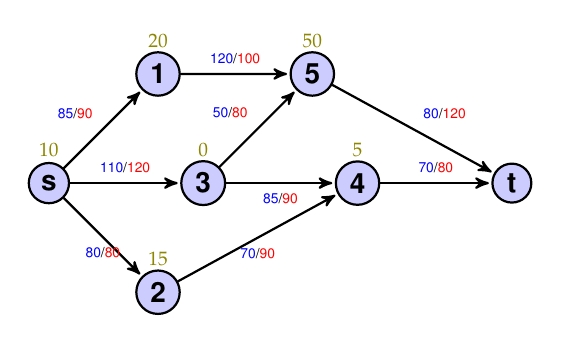
\begin{tikzpicture}[->,>=stealth',shorten >=1pt,auto,node distance=2.8cm,scale=0.7, every node/.style={scale=0.7}, thick,main node/.style={circle,fill=blue!20,draw,font=\sffamily\Large\bfseries},
highlight/.style={ultra thick,draw=blue, text=blue}]

  \node[main node] (s) {s};
  \node (stop) at ($(s) + (90:.6)$) {\textcolor{olive}{10}};

  \node[main node] (1) [above right of=s] {1};
  \node (1top) at ($(1) + (90:.6)$) {\textcolor{olive}{20}};

  \node[main node] (2) [below right of=s] {2};
  \node (2top) at ($(2) + (90:.6)$) {\textcolor{olive}{15}};

  \node[main node] (3) [right of=s] {3};
  \node (3top) at ($(3) + (90:.6)$) {\textcolor{olive}{0}};

  \node[main node] (4) [right of=3] {4};
  \node (4top) at ($(4) + (90:.6)$) {\textcolor{olive}{5}};

  \node[main node] (5) [right of=1] {5};
  \node (5top) at ($(5) + (90:.6)$) {\textcolor{olive}{50}};

  \node[main node] (t) [right of=4] {t};

  \path[every node/.style={font=\sffamily\tiny}]
      (s) edge[onslide={<3>, highlight}] node {\textcolor{blue}{85}/\textcolor{red}{90}} (1)
      (s) edge[onslide={<4>, highlight}] node [below] {\textcolor{blue}{80}/\textcolor{red}{80}} (2)
      (s) edge[onslide={<5>, highlight}] node {\textcolor{blue}{110}/\textcolor{red}{120}} (3)

      (1) edge[onslide={<7>, highlight}] node {\textcolor{blue}{120}/\textcolor{red}{100}} (5)

      (2) edge[onslide={<12>, highlight}] node [below] {\textcolor{blue}{70}/\textcolor{red}{90}} (4)

      (3) edge[onslide={<10>, highlight}] node [below] {\textcolor{blue}{85}/\textcolor{red}{90}} (4)
      (3) edge[onslide={<9>, highlight}] node {\textcolor{blue}{50}/\textcolor{red}{80}} (5)

      (4) edge[onslide={<14>, highlight}] node {\textcolor{blue}{70}/\textcolor{red}{80}} (t)

      (5) edge[onslide={<16>, highlight}] node {\textcolor{blue}{80}/\textcolor{red}{120}} (t);

 %onslide={<2>, highlight}
\end{tikzpicture}

\only<1>{Edge weights:
\begin{itemize}
  \item \textcolor{blue}{distance (km)}
  \item \textcolor{red}{speed limit(km/hr)}
\end{itemize}
Vertex weights:\\
\begin{itemize}
  \item \textcolor{olive}{charging speed (kW)}
\end{itemize}
}

\only<2>{
$Q=\{s\}$\\
Best: s
}
\only<3>{
Driving: 90km/hr: 0.94 hr\\
Charge and drive: Same
}
\only<4>{
Driving: 80km/hr: 1hr\\
Charge and drive: Same
}
\only<5>{
Driving: 120km/hr: 0.92hr\\
Charge and drive: Same
}
\only<6>{
$Q=\{1,3,2\}$\\
Best: 1
}
\only<7>{
Driving: 71.1km/hr: 1.7 hr\\
Charge and drive: 88.1km/hr: 1.6 hr
}
\only<8>{
$Q=\{3,2,5\}$\\
Best: 3
}
\only<9>{
Driving: Not possible!\\
Charge and drive: Not possible!
}
\only<10>{
Driving: Not possible\\
Charge and drive: Not possible!
}
\only<11>{
$Q=\{2,5\}$\\
Best: 2
}
\only<12>{
Driving: 90km/hr: 0.8hr\\
Charge and drive: Same
}
\only<13>{
$Q=\{5,4\}$\\
Best: 4
}
\only<14>{
Driving: Not possible\\
Charge and drive: 58.6km/hr: 1.2hr\\
Uses previous charging station of 15kW!
}
\only<15>{
$Q=\{5\}$\\
Best: 5
}
\only<16>{
Driving: Not possible\\
Charge and drive: 120km/hr: 1.2hr}
\only<17>{
  Conclusion
  \begin{itemize}
    \item Greedy path: $\langle s,2,4,t \rangle$, 3 hours
    \item Optimal path: $\langle s,3,5,t\rangle$, 2.8 hours
  \end{itemize}
}



\column{0.45\textwidth}

\only<1>{Paths:\\
$\langle s,1,5,t\rangle$: 285km, 2.8hr \\
$\langle s,3,4,t\rangle$: 265km, 2.7hr\\
$\langle s,3,5,t\rangle$: 240km, 2.2hr\\
$\langle s,2,4,t\rangle$: 220km, 2.7hr}
\only<2->{
  \begin{tabular}{| c | c | c | c | c |}
    \hline
    & $\pi$ & time & bat\\ \hline
    s& & 0 &  50 \\ \hline
    \only<2>{1& & &\\ \hline
    2& & &\\ \hline
    3& & &\\ \hline
    4& & &\\ \hline
    5& & &\\ \hline
    t& & &\\ \hline
    }\only<3>{1& s & 0.9 & 27.1\\ \hline
    2& & &\\ \hline
    3& & &\\ \hline
    4& & &\\ \hline
    5& & &\\ \hline
    t& & &\\ \hline
    }\only<4>{1& s & 0.9 & 27.1\\ \hline
    2& s & 1 & 30.4\\ \hline
    3& & &\\ \hline
    4& & &\\ \hline
    5& & &\\ \hline
    t& & &\\ \hline
    }\only<5-6>{1& s & 0.9 &27.1\\ \hline
    2& s & 1 & 30.4\\ \hline
    3& s & 0.9 & 9.8\\ \hline
    4& & &\\ \hline
    5& & &\\ \hline
    t& & &\\ \hline
    }\only<7-11>{1& s & 0.9 & 27.1\\ \hline
    2& s & 1  & 30.4\\ \hline
    3& s & 0.9 & 9.8\\ \hline
    4& & &\\ \hline
    5& 1 & 2.5 &  0\\ \hline
    t& & &\\ \hline
    }\only<12-13>{1& s & 0.9 & 27.1\\ \hline
    2& s & 1 & 30.4\\ \hline
    3& s & 0.9 & 9.8\\ \hline
    4& 2 & 1.8 & 11.6\\ \hline
    5& 1 & 2.5 & 0\\ \hline
    t& & &\\ \hline
    }\only<14->{1& s & 0.9 & 27.1\\ \hline
    2& s & 1 & 30.4\\ \hline
    3& s & 0.9 & 9.8\\ \hline
    4& 2 & 1.8 & 11.6\\ \hline
    5& 1 & 2.5 & 0\\ \hline
    t & 4 & 3 & 0\\ \hline
    }
  \end{tabular}
}

\end{columns}
\end{frame}


\section{A-NIDS}

\begin{frame}Anomaly based Network Intrusion Detection System (A-NIDS)

\begin{itemize}
	\item Statistical based
		\begin{itemize}
			\item Univariate
			\item Multivariate
		\end{itemize}
	\item Knowledge based
	\item \textbf{Machine learning based}
\end{itemize}

Exploiting Communication Regularities

\begin{itemize}
	\item Learn the normal sequences of messages on a network
	\item Build a model describing these sequences
\end{itemize}
\end{frame}

\begin{frame}Machine Learning

\begin{itemize}
	\item Bayesian networks
	\item \textbf{Markov models}
	\item Neural networks
	\item Fuzzy logic
	\item Genetic algorithm
	\item Etc.
\end{itemize}	
\end{frame}



\section{Bayesian Networks}


\subsection{The Model}
\begin{frame}


\end{frame}

\section{Hidden Markov Model}

\begin{frame}Hidden Markov Model
\begin{figure}
\centering
	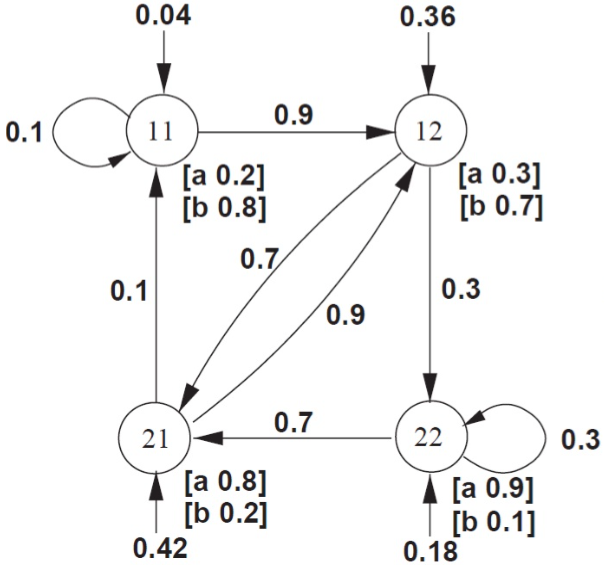
\includegraphics[scale=0.28]{./content/hmm}
	\caption{PAutomaC: a PFA/HMM Learning Competition, Sicco Verwer et al., 2012}
\end{figure}
\end{frame}


\begin{frame}Hidden Markov Model - Urn and Ball
\begin{figure}
\centering
	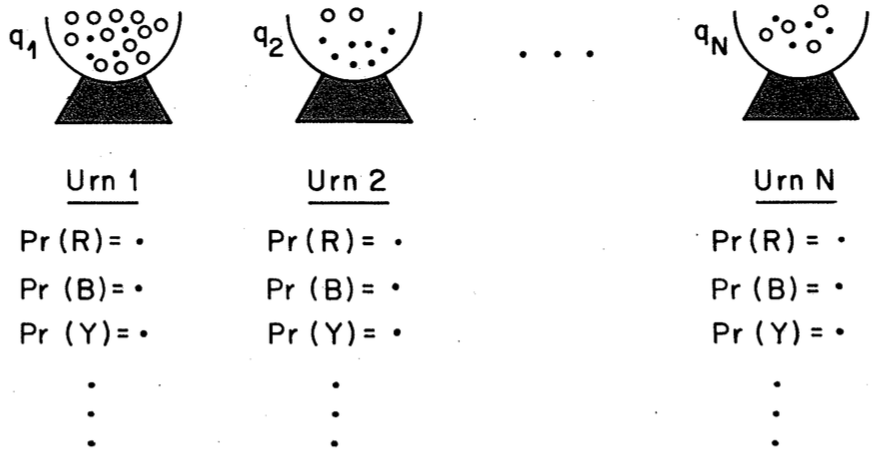
\includegraphics[scale=0.28]{./content/urn}
	\caption{An Introduction to Hidden Markov Models, L. R. Rabiner B. H. juang, 1986}
\end{figure}
\end{frame}


\begin{frame}Hidden Markov Model
	\begin{itemize}
		\item $T$ = length of observation sequence
		\item $N$ = number of states in the model
		\item $M$ = number of observation symbols
		\item $Q$ = \{$q_1, q_2,...,q_N$\}, states
		\item $V$ = \{$v_1, v_2,...,v_M$\}, \\
		observation symbols
		\item $A$ = \{$a_{ij}$\}, $a_{ij}$ = $Pr(q_j$, at $t + 1 | q_i$ at $t)$, \\
		state transition probability distribution
		\item $B$ = \{$b_j(k)$\}, $b_j(k)$ = $Pr(v_k$ at $t  | q_j$ at $t)$, \\
		observation symbol probability distribution
		\item $\pi$ = \{$\pi_i$\}, $\pi_i$ = $Pr(q_i$ at $t = 1)$, \\
		initial state distribution
		\item $\lambda$ = ($A$, $B$, $\pi$), the HMM
	\end{itemize}
	
	\begin{tikzpicture}[remember picture,overlay]  
      \node [xshift=-2.7cm,yshift=-3cm] at (current page.north east)
    {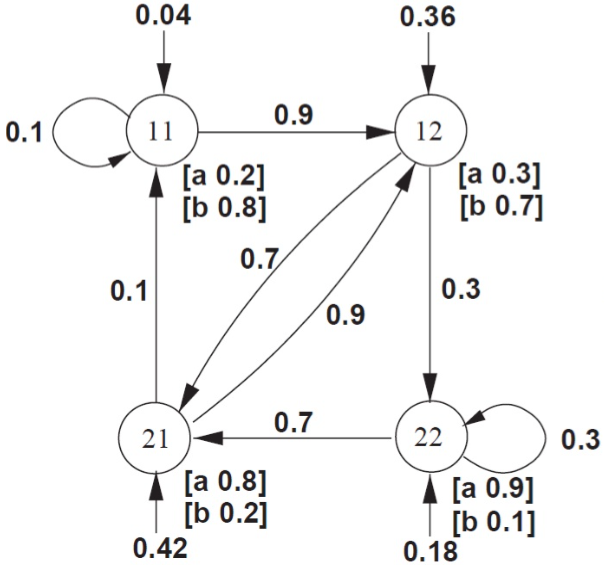
\includegraphics[scale=0.2]{./content/hmm}};
	\end{tikzpicture}		
\end{frame}

\end{document}



















